\documentclass[a4paper]{article}
\usepackage[UTF8]{ctex}
\usepackage{geometry}
\usepackage{graphicx}
\usepackage{url}
\usepackage{multirow}
\usepackage{array}
\usepackage{booktabs}
\usepackage{url}
\usepackage{enumitem}
\usepackage{graphicx}
\usepackage{float}
\usepackage{amssymb}
\usepackage{amsmath}
\usepackage{subfig}
\usepackage{longtable}
\usepackage{pifont}
\usepackage{color}

\allowdisplaybreaks

\geometry{a4paper, scale=0.78}

% \begin{figure}[H]
%     \centering
%     \includegraphics[width=.55\textwidth]{E.png}
%     \caption{矩阵与列向量的乘法}
%     \label{fig:my_label_1}
% \end{figure}

% \left\{
% \begin{array}{ll}
%       x+2x+z=2 & \\
%       3x+8y+z=12 & \\
%       4y+z=2
% \end{array}
% \right.

% \begin{enumerate}[itemindent = 1em, itemsep = 0.4pt, parsep=0.5pt, topsep = 0.5pt]

% \end{enumerate}

%\stackrel{a}{\longrightarrow}

%\underbrace{}_{} %下括号

%\tableofcontents %目录,并且目录页不记录页码
% \tableofcontents
% \newpage
% \setcounter{page}{1} %new page
% \clearpage

\title{Hidden Markov Model 04 Decoding}
\author{Chen Gong}
\date{10 January 2020}

\begin{document}
\maketitle
Decoding问题可被我们描述为:
\begin{equation}
    \hat{I} = \arg\max_{I} P(I|O,\lambda)
\end{equation}

也就是在给定观察序列的情况下,寻找最大概率可能出现的隐概率状态序列。也有人说Decoding问题是预测问题,但是实际上这样说是并不合适的。预测问题应该是,$P(o_{t+1}|o_1,\cdots,o_t)$和$P(i_{t+1}|o_1,\cdots,o_t)$,这里的$P(i_{1},\cdots,i_t|o_1,\cdots,o_t)$看成是预测问题显然是不合适的。

\section{Decoding Problem}
下面我们展示一下Hidden Markov Model的拓扑模型:
\begin{figure}[H]
    \centering
    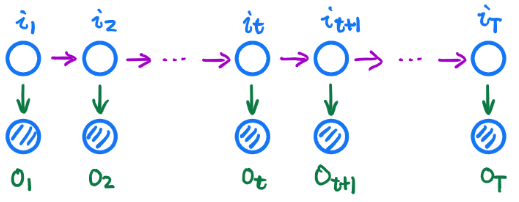
\includegraphics[width=.5\textwidth]{微信图片_20200109224115.png}
    \caption{Hidden Markov Model的拓扑模型}
    \label{fig:my_label_1}
\end{figure}

这里实际上就是一个动态规划问题,这里的动态规划问题实际上就是最大概率问题,只不过将平时提到的最大距离问题等价于最大概率问题,理论上都是一样的。每个时刻都有$N$个状态,所有也就是从$N^T$个可能的序列中找出概率最大的一个序列,实际上就是一个动态规划问题,如下图所示:
\begin{figure}[H]
    \centering
    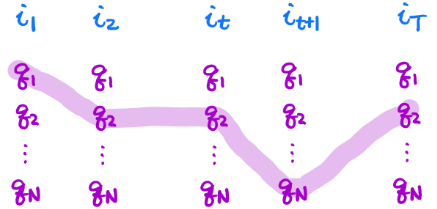
\includegraphics[width=.5\textwidth]{微信图片_20200109225254.png}
    \caption{Decoding的动态规划问题}
    \label{fig:my_label_1}
\end{figure}

我们假设:
\begin{equation}
    \delta_t(i) = \max_{i_1,\cdots,i_{t-1}} P(o_1,\cdots,o_t,i_1,\cdots,i_{t-1},i_t=q_i)
\end{equation}

这个等式是什么意思呢?也就是当$t$个时刻是$q_i$,前面$t-1$个随便走,只要可以到达$q_i$这个状态就行,而从中选取概率最大的序列。我们下一步的目标就是在知道$\delta_t(i)$的情况下如何求$\delta_t(i+1)$,那么这样就能通过递推来求得知道最后一个状态下概率最大的序列。$\delta_t(i+1)$的求解方法如下所示:
\begin{figure}[H]
    \centering
    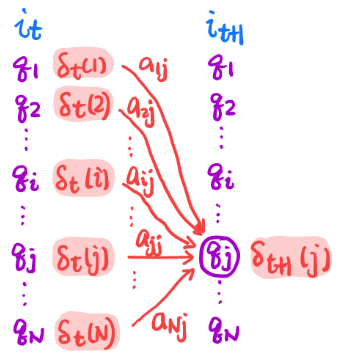
\includegraphics[width=.35\textwidth]{微信图片_20200109230705.png}
    \caption{根据$\delta_t(i)$求解$\delta_t(i+1)$的方法示意图}
    \label{fig:my_label_1}
\end{figure}

所以,
\begin{equation}
\begin{split}
    \delta_{t+1}(j) 
    = & \max_{i_1,\cdots,i_{t}} P(o_1,\cdots,o_{t+1},i_1,\cdots,i_{t},i_{t+1}=q_j) \\
    = & \max_{i_1,\cdots,i_{t}} \delta_t(i)\cdot a_{ij}\cdot b_j(o_{t+1}) \\
\end{split}
\end{equation}

这就是Viterbi算法,但是这个算法最后求得的是一个值,没有办法求得路径,如果要想求得路径,我们需要引入一个变量:
\begin{equation}
    \varphi_{t+1}(j) = \arg\max_{1\leq i \leq N}\delta_t(i)\cdot a_{ij}\cdot b_j(o_{t+1})
\end{equation}

这个函数用来干嘛的呢?他是来记录每一次迭代过程中经过的状态的index。这样我们最终得到的$\{ \varphi_1,\varphi_2,\cdots,\varphi_T \}$,就可以得到整个路径了。

\end{document}
